\chapter{Knowledge and the Transformation of Man}

This chapter follows the first San Diego conversation between J. Krishnamurti and Allan W. Anderson on knowledge and the transformation of man. There is no blackboard mathematics in the lecture, and no validated screenshot remains as visual evidence. The formal structure below is therefore deliberately modest: we use equations only as disciplined notation for the order of the inquiry. The point is not to mathematize Krishnamurti's language, but to make visible the chain by which the lecture moves from world disorder, to the divided human being, to knowledge as the past, and finally to the question of freedom from the known.

\section{The Disorder That Raises the Question}

The lecture does not begin with an abstract definition of happiness, knowledge, or transformation. It begins with the state of the world. Krishnamurti points to degeneration in culture, art, literature, and religion; to the mere acceptance of authority and belief; to confusion, misery, sorrow, and the incapacity of institutions to reach the root of human disorder.

That opening is essential. If we remove it, the later question about knowledge becomes an academic exercise. In the lecture it is not academic. The question is forced by what we see: a world in disorder, and a human mind which has produced and continues to sustain that disorder.

The first reduction is from the world problem to the human problem. The transformation of society is not assigned to the mass, the priest, the church, the temple, the politician, the scientist, or the businessman. It is placed on the human being who sees the confusion and asks whether radical transformation is possible.

We can write the first movement schematically as
\begin{equation}
\mathrm{world\ disorder}
\longrightarrow
\mathrm{question\ of\ human\ transformation}.
\end{equation}
This is not a causal law. It is the order of attention in the lecture. First one sees the disorder; then one asks what in the human being must change.

Krishnamurti also distinguishes deep concern from superficial concern. Energy, pollution, and practical public problems are not denied, but they are treated as superficial if they do not reach the human mind which is destroying the world. The inquiry therefore turns from external symptoms to the structure of the human mind itself.

\section{Individual, Human Being, Whole}

Anderson first formulates the issue in terms of the individual. Krishnamurti immediately corrects the word. In ordinary speech, an individual is a countable person, one among many. But the word also carries the sense of the undivided. In that deeper sense, a fragmented human being is not yet an individual.

The distinction is important enough to make explicit:
\begin{align}
\mathrm{individual}_{\mathrm{ordinary}}
&= \mathrm{one\ separate\ person},\\
\mathrm{individual}_{\mathrm{qualitative}}
&= \mathrm{undivided,\ whole,\ unfragmented}.
\end{align}

The second line is the one Krishnamurti wants to recover. A human being may have a name, a house, a bank account, and a social identity, yet still be inwardly fragmented. Such a person is not an individual in the sense that matters for this inquiry.

The word ``whole'' then opens into a cluster of meanings. Krishnamurti links it with sanity, health, and holiness. This is not a doctrinal claim about belonging to a religion. It is a linguistic and existential point: the human being who is whole is not divided against himself, and therefore is not merely a social unit seeking private security.

\begin{definition}
In this chapter, a whole human being means a human being who is not inwardly fragmented by contradiction, division, and conflicting desire. The term is used in Krishnamurti's qualitative sense: whole, sane, healthy, and therefore holy.
\end{definition}

Responsibility follows from this. It is not merely my private responsibility or your private responsibility. It belongs to each human being because the disorder is not outside the human field. Krishnamurti gives responsibility a precise tone: it implies attention, care, and diligence, not negligence.

\subsection{Question \& Answer}

\paragraph{Question.}
If the change must begin with each human being, does that mean the problem is private, separate, and individualistic?

\paragraph{Answer.}
No. The lecture corrects that misunderstanding at once. The human being is not an isolated psychological island. Wherever people live, Krishnamurti says, they face sorrow, fear, livelihood, relationship, survival, overpopulation, life, and death. These are not eastern or western problems in essence. They are human problems.

So the responsibility of each human being is not a retreat into private self-concern. It is responsibility in relation to the whole of mankind. The lecture is careful here: it refuses both collectivist evasion and private isolation. The human being must begin, but the human being is already implicated in the whole.

\section{The Human Being Is the World}

The next turn is the central structural claim of the conversation:
\begin{equation}
\mathrm{human\ being}
\leftrightarrow
\mathrm{world}.
\end{equation}
The arrow is not meant as a mechanical equation. It says that the human being and the world are not two separate compartments. Human beings have created the society in which they live: through greed, anger, violence, brutality, pettiness, ambition, and fear. At the same time, each human being is shaped by the culture into which he or she is born.

Krishnamurti's formulation is stronger than saying that the individual influences society and society influences the individual. He says that the human being is the world and the world is the human being. If that is seen, then the question of transformation cannot be displaced into external reform alone.

\begin{figure}
\centering
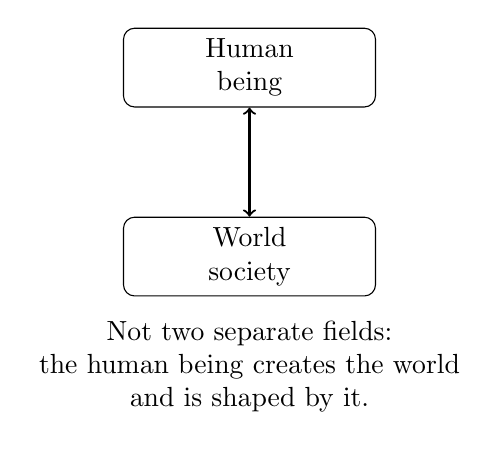
\begin{tikzpicture}[x=1cm,y=1cm]
\node[draw, rounded corners, minimum width=3.2cm, minimum height=1.0cm, align=center] (h) at (0,1.2) {Human\\being};
\node[draw, rounded corners, minimum width=3.2cm, minimum height=1.0cm, align=center] (w) at (0,-1.2) {World\\society};
\draw[<->, thick] (h) -- (w);
\node[align=center, text width=5.4cm] at (0,-2.6) {Not two separate fields:\\the human being creates the world\\and is shaped by it.};
\end{tikzpicture}
\caption{A conceptual reconstruction of the lecture's non-separation claim.}
\end{figure}

This is why changing the social structure by itself is not enough. Krishnamurti mentions the old hope that changing the environment will change the human being. The lecture rejects that as insufficient. Structures may change, and they may polish the surface, but the root remains untouched if the mind that produces disorder remains the same.

The order is therefore not
\begin{equation}
\mathrm{change\ society}
\longrightarrow
\mathrm{change\ human\ being}.
\end{equation}
Nor is it a private sequence in which a separate individual perfects himself and only later affects the world. The lecture instead proposes a non-separate relation:
\begin{equation}
\mathrm{root\ change\ in\ the\ human\ being}
\longleftrightarrow
\mathrm{change\ in\ the\ world}.
\end{equation}

This is why Anderson calls attention to a non-temporal relation. It is not an if-then sequence: first an inward event, later an outward result. The inward and outward are not two independent orders.

\section{Change at the Root}

The conversation then examines the word revolution. In ordinary political language, revolution may mean overthrowing a government. Krishnamurti distinguishes that from psychological revolution. The lecture is not concerned with a merely bloody or outward revolution, but with a revolution in the very structure and nature of thought.

A useful table is the following:
\begin{table}
\centering
\begin{tabular}{|p{0.28\linewidth}|p{0.56\linewidth}|}
\hline
Outward revolution & Change of government, structure, policy, or social arrangement. It may be violent or ideological, but it need not touch the root of the mind.\\
\hline
Gradual evolution & Slow modification through time. In the lecture, this is treated as endless postponement when applied to psychological transformation.\\
\hline
Psychological revolution & A fundamental change in the way the human being thinks, behaves, conducts himself, and functions.\\
\hline
\end{tabular}
\caption{Three senses of change distinguished in the dialogue.}
\end{table}

The lecture momentarily uses the word ``instant,'' but Krishnamurti is cautious about it. He does not want the word to suggest a dramatic event that happens magically. At the same time, he rejects gradual psychological evolution as the answer. The point is not speed measured by a clock. The point is freedom from the psychological structure of postponement.

We can mark the distinction this way:
\begin{align}
\mathrm{surface\ reform}
&\ne
\mathrm{root\ transformation},\\
\mathrm{gradual\ psychological\ progress}
&\ne
\mathrm{freedom\ from\ the\ old}.
\end{align}

This is one of the places where the chapter must not flatten the repetition. Krishnamurti returns several times to the same point because the common mind wants to escape into reform, time, theory, or method. He keeps bringing the inquiry back to the root.

\section{Division and Conflict}

The next step is division. The world is divided into East and West, religions, nationalities, ideologies, and opposing groups. We also divide ourselves inwardly and socially: Christian and non-Christian, Hindu and Muslim, capitalist and socialist, we and they, I and you.

Krishnamurti gives the relation with almost law-like force:
\begin{equation}
\mathrm{Division}
\longrightarrow
\mathrm{Conflict}.
\end{equation}
We should not turn this into a theorem. It is a central observation in the dialogue. Where there is division, there is opposition; where there is opposition, there is conflict.

The deeper point is that division is often created in the search for security. The mind divides in order to protect itself: my nation, my religion, my belief, my group, my knowledge. But the result is insecurity. The very movement that seeks safety produces conflict.

\begin{figure}
\centering
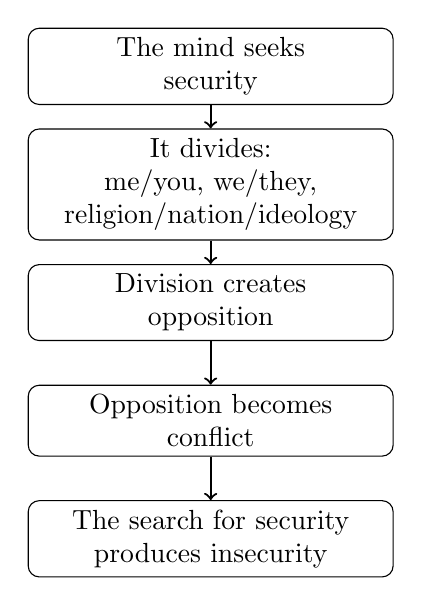
\begin{tikzpicture}[x=1cm,y=1cm]
\node[draw, rounded corners, align=center, text width=4.4cm] (a) at (0,3.0) {The mind seeks\\security};
\node[draw, rounded corners, align=center, text width=4.4cm] (b) at (0,1.5) {It divides:\\me/you, we/they,\\religion/nation/ideology};
\node[draw, rounded corners, align=center, text width=4.4cm] (c) at (0,0) {Division creates\\opposition};
\node[draw, rounded corners, align=center, text width=4.4cm] (d) at (0,-1.5) {Opposition becomes\\conflict};
\node[draw, rounded corners, align=center, text width=4.4cm] (e) at (0,-3.0) {The search for security\\produces insecurity};
\draw[->, thick] (a) -- (b);
\draw[->, thick] (b) -- (c);
\draw[->, thick] (c) -- (d);
\draw[->, thick] (d) -- (e);
\end{tikzpicture}
\caption{A transcript-backed reconstruction of the movement from security-seeking division to conflict.}
\end{figure}

Anderson briefly brings in scriptural language: the one doing the truth is coming to the light, not doing one thing first and later receiving another. Krishnamurti accepts the general direction: living truth is not a static state and not an intellectual acceptance. The important structural point is concurrency. Action and understanding are not arranged as a bargain in time.

\begin{equation}
\mathrm{Action}
\parallel
\mathrm{Understanding}.
\end{equation}
The symbol here is only shorthand. It means that, in the lecture's terms, action and understanding are not treated as an if-then sequence.

\subsection{Question \& Answer}

\paragraph{Question.}
Can the human mind, conditioned for millennia and loaded with knowledge, regenerate now?

\paragraph{Answer.}
That is the hinge of the lecture. Krishnamurti asks whether the mind can be free to renew itself now. The phrase ``reincarnate now'' should be heard carefully: in this conversation it points to immediate regeneration, not to a doctrine about rebirth. The obstacle is not lack of information. It is the mind's dependence on division, tradition, and accumulated knowledge.

The answer is not yet a method. The lecture does not say: do these steps and you will be transformed. It sharpens the question. If the mind is divided, if it has sought security through separation, and if its knowledge is an accumulation from the past, then what place has knowledge in transformation?

\section{Knowledge, Time, and the Past}

At this point the lecture arrives at its main analytic movement. Krishnamurti asks what it means to know. Anderson offers a stricter philosophical phrase: knowledge as apprehension of what is. Krishnamurti turns instead to what is generally accepted as knowledge: experience.

The chain is direct:
\begin{equation}
\mathrm{Experience}
\longrightarrow
\mathrm{Mark}
\longrightarrow
\mathrm{Memory}
\longrightarrow
\mathrm{Knowledge}.
\end{equation}
Experience leaves a mark. That mark becomes memory. Memory is accumulated as knowledge.

Then comes the decisive identity:
\begin{align}
\mathrm{Knowledge} &= \mathrm{the\ known},\\
\mathrm{the\ known} &= \mathrm{the\ past},\\
\therefore\quad \mathrm{Knowledge} &= \mathrm{the\ past}.
\end{align}

This is not a denial of practical knowledge. Krishnamurti explicitly says that knowledge has its place. We must know where we are going physically; we need technological, practical, and ordinary functional knowledge. The question is what place that knowledge has in transforming a mind that is brutal, violent, petty, selfish, greedy, and ambitious.

\begin{table}
\centering
\begin{tabular}{|p{0.30\linewidth}|p{0.54\linewidth}|}
\hline
Practical knowledge & Knowing how to navigate, build, speak, repair, calculate, remember facts, and function in the practical order. This has its place.\\
\hline
Psychological knowledge & The accumulated image of oneself and another: insult, praise, hurt, flattery, fear, tradition, belief, and remembered injury. This carries the past into relationship.\\
\hline
\end{tabular}
\caption{The lecture preserves practical knowledge while questioning psychological dependence on the known.}
\end{table}

\subsection{Question \& Answer}

\paragraph{Question.}
If knowledge has a place, why does Krishnamurti ask whether transformation is free from knowledge and time?

\paragraph{Answer.}
Because the issue is not practical knowledge but psychological continuity. Practical knowledge can function in the present, but it has its roots in the past. When that past becomes the measure of present relationship, the present is no longer met directly.

The problem can be written as an update rule:
\begin{equation}
\mathrm{new\ encounter}_{n+1}
\longmapsto
\mathrm{interpretation}\bigl(\mathrm{new\ encounter}_{n+1}\,;\,\mathrm{memory}_{n}\bigr).
\end{equation}
The next encounter is translated in terms of the old. In Krishnamurti's words, that means the experience is never new. The old has already entered as the interpreter.

\subsection{A Worked Conceptual Derivation}

We can spell out the lecture's argument as a short derivation.

\begin{enumerate}
\item A human being has an experience.
\item The experience leaves a mark.
\item The mark is retained as memory.
\item Memory is accumulated as knowledge.
\item Knowledge is the known.
\item The known is the past.
\item Therefore psychological knowledge carries the past into the present.
\item If the past interprets the present, the present is not met directly.
\end{enumerate}

In compact notation:
\begin{align}
E &\longrightarrow M,\\
M &\longrightarrow K,\\
K &= P,\\
P + \mathrm{present\ encounter}
&\longrightarrow
\mathrm{old\ interpretation}.
\end{align}
Here \(E\) means experience, \(M\) means mark or memory, \(K\) means knowledge, and \(P\) means the past. These symbols are only bookkeeping. They keep the order of the lecture visible.

\section{Image, Relationship, and Registration}

The lecture now becomes intensely concrete. Krishnamurti says: I met you yesterday, and there is an image of you in my mind. That image meets you the next day. The image meets you; I do not meet you.

This is the crucial passage from knowledge to relationship. Knowledge is no longer merely an epistemological term. It becomes image, and image becomes the obstruction between human beings.

The lecture's equivalence is:
\begin{equation}
\mathrm{Image}
=
\mathrm{Knowledge}
=
\mathrm{Tradition}
=
\mathrm{Past}.
\end{equation}
Again, this is not formal psychology. It is the vocabulary of the conversation. Image is the past carried as knowledge into relationship.

\begin{figure}
\centering
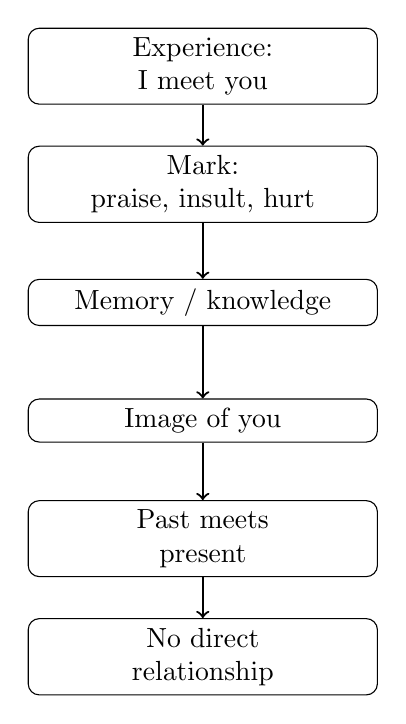
\begin{tikzpicture}[x=1cm,y=1cm]
\node[draw, rounded corners, align=center, text width=4.2cm] (e) at (0,4.5) {Experience:\\I meet you};
\node[draw, rounded corners, align=center, text width=4.2cm] (m) at (0,3.0) {Mark:\\praise, insult, hurt};
\node[draw, rounded corners, align=center, text width=4.2cm] (k) at (0,1.5) {Memory / knowledge};
\node[draw, rounded corners, align=center, text width=4.2cm] (i) at (0,0) {Image of you};
\node[draw, rounded corners, align=center, text width=4.2cm] (p) at (0,-1.5) {Past meets\\present};
\node[draw, rounded corners, align=center, text width=4.2cm] (r) at (0,-3.0) {No direct\\relationship};
\draw[->, thick] (e) -- (m);
\draw[->, thick] (m) -- (k);
\draw[->, thick] (k) -- (i);
\draw[->, thick] (i) -- (p);
\draw[->, thick] (p) -- (r);
\end{tikzpicture}
\caption{The lecture's practical chain from experience to image and blocked relationship.}
\end{figure}

The problem is not whether the brain records. Krishnamurti says the brain records all the time. The question is subtler: can the brain record what is necessary and not let the record move into psychological interference?

\subsection{Question \& Answer}

\paragraph{Question.}
How can the mind record without being trapped by what it records?

\paragraph{Answer.}
The lecture does not give a technique. It refuses the easy answer that one can simply negate the record by will. If you insult me or praise me, the event may leave a mark. If that mark becomes an image, then the next meeting is shaped by memory. The image meets you; relationship is lost.

So the question becomes precise:
\begin{equation}
\mathrm{recording}
\;\not\longrightarrow\;
\mathrm{psychological\ image}.
\end{equation}
This is the open problem carried into the next conversation. Krishnamurti asks how the mind, which functions on knowledge and records all the time, can be free of knowledge in the psychological sense.

\section{The Word Is Not the Thing}

The final movement returns to theory, religion, and tradition. Religion as it commonly exists is described as propaganda, belief, idolatry, fear, division, and the acceptance of ideas put out by thought. In that form, religion is not transformation; it is the denial of truth.

Anderson introduces theory in the Greek sense of seeing or spectacle. Krishnamurti keeps pressing the distinction between living fact and description. Theories may have their intellectual place, but they do not transform a human being who is actually living.

The lecture's last major negations are:
\begin{align}
\mathrm{Word} &\ne \mathrm{Thing},\\
\mathrm{Description} &\ne \mathrm{Described}.
\end{align}
This is the same structure as the earlier critique of knowledge. When the description replaces what is, action does not take place. When one is confronted with what is, action becomes possible.

\begin{proposition}
In the order of this lecture, transformation is blocked when the mind substitutes description, theory, belief, or image for direct contact with what is.
\end{proposition}

\begin{proof}
The lecture has already shown the pattern. Experience leaves a mark; the mark becomes memory; memory becomes knowledge; knowledge becomes image; image meets the present. In the same way, a word, theory, or belief may stand between the human being and the fact. When the mind lives through that substitute, it repeats the past. When it is confronted with what is, the possibility of action appears.
\end{proof}

Krishnamurti closes by gathering the open questions. Can there be freedom from knowledge, while knowledge still has its practical place? Can there be freedom from tradition as knowledge? Can there be freedom from the separative outlook of me and you, we and they, Christian and non-Christian? These are not rhetorical flourishes. They define the next step of the inquiry.

\section{Summary}

The conversation begins with the disorder of the world and refuses to treat that disorder as merely external. The human being has made the world, and the world has shaped the human being. Therefore the root of transformation cannot be found in social structure alone, nor in gradual psychological improvement, nor in a theory about change.

The lecture's conceptual spine is:
\begin{equation}
\mathrm{Experience}
\longrightarrow
\mathrm{Mark}
\longrightarrow
\mathrm{Memory}
\longrightarrow
\mathrm{Knowledge}
\longrightarrow
\mathrm{Image}
\longrightarrow
\mathrm{blocked\ relationship}.
\end{equation}
Knowledge has its practical place, but psychological knowledge is the past. When the past meets the present as image, relationship is distorted. When division is taken as security, conflict follows.

The chapter therefore ends where the lecture ends: with the question of actual freedom from the known. Not verbal freedom, not speculative freedom, not the description of freedom, but whether the mind can be free from the old movement of knowledge, image, tradition, and division.